\documentclass[tikz,border=10pt]{standalone}

\begin{document}
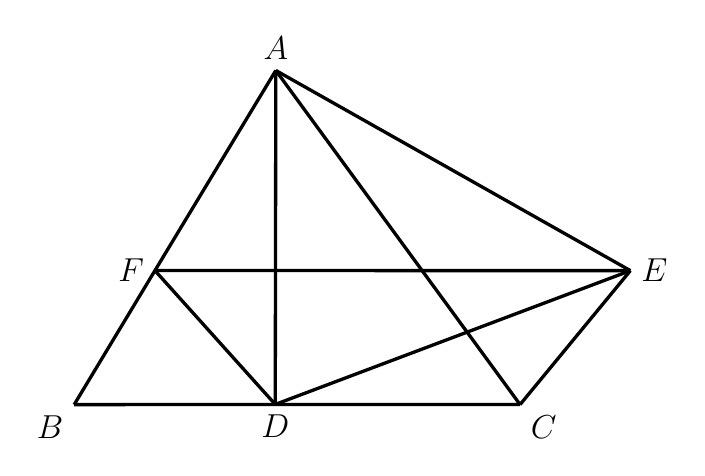
\begin{tikzpicture}[line width=1.2pt, line join=round, every node/.style={font=\fontsize{12}{14.4}\selectfont}]
\coordinate (A) at (-0.993,2.128);
\coordinate (B) at (-3.554,-2.116);
\coordinate (C) at (2.109,-2.115);
\coordinate (D) at (-1.000,-2.113);
\coordinate (F) at (-2.528,-0.413);

  
  \coordinate (E) at (3.510,-0.414);

  
  \draw (A) -- (F) -- (B);
  
  \draw (B) -- (D) -- (C);
  
  \draw (A) -- (D);
  
  \draw (A) -- (C);
  
  \draw (A) -- (E);
  
  \draw (F) -- (E);
  
  \draw (F) -- (D);
  
  \draw (D) -- (E);
  
  \draw (C) -- (E);

  
  \node[above] at (A) {$A$};
  \node[below left] at (B) {$B$};
  \node[below right] at (C) {$C$};
  \node[below] at (D) {$D$};
  \node[right] at (E) {$E$};
  \node[left] at (F) {$F$};
\end{tikzpicture}
\end{document}